\documentclass{beamer}
\usepackage[english,russian]{babel}
\usepackage[utf8]{inputenc}
\usepackage{amsmath}
\usepackage{hyperref}
\usetheme{Warsaw}
\usepackage{listings}
\usepackage{xcolor}
\usepackage{tikz}
\usetikzlibrary{graphs}
\usepackage{algpseudocode}

\lstset{
    frame=tb,
    tabsize=4,
    showstringspaces=false,
    numbers=left,
    commentstyle=\color{green},
    keywordstyle=\color{blue},
    stringstyle=\color{red},
    emph={baz},
    emphstyle=\textbf
}

\begin{document}

\title{Задачи разрешимости логических формул и приложения\newline Лекция 5. Логики равенства и неинтерпритируемых функций}
\author{Роман Холин}
\institute{Московский государственный университет}
\date{Москва, 2022}

\begin{frame}
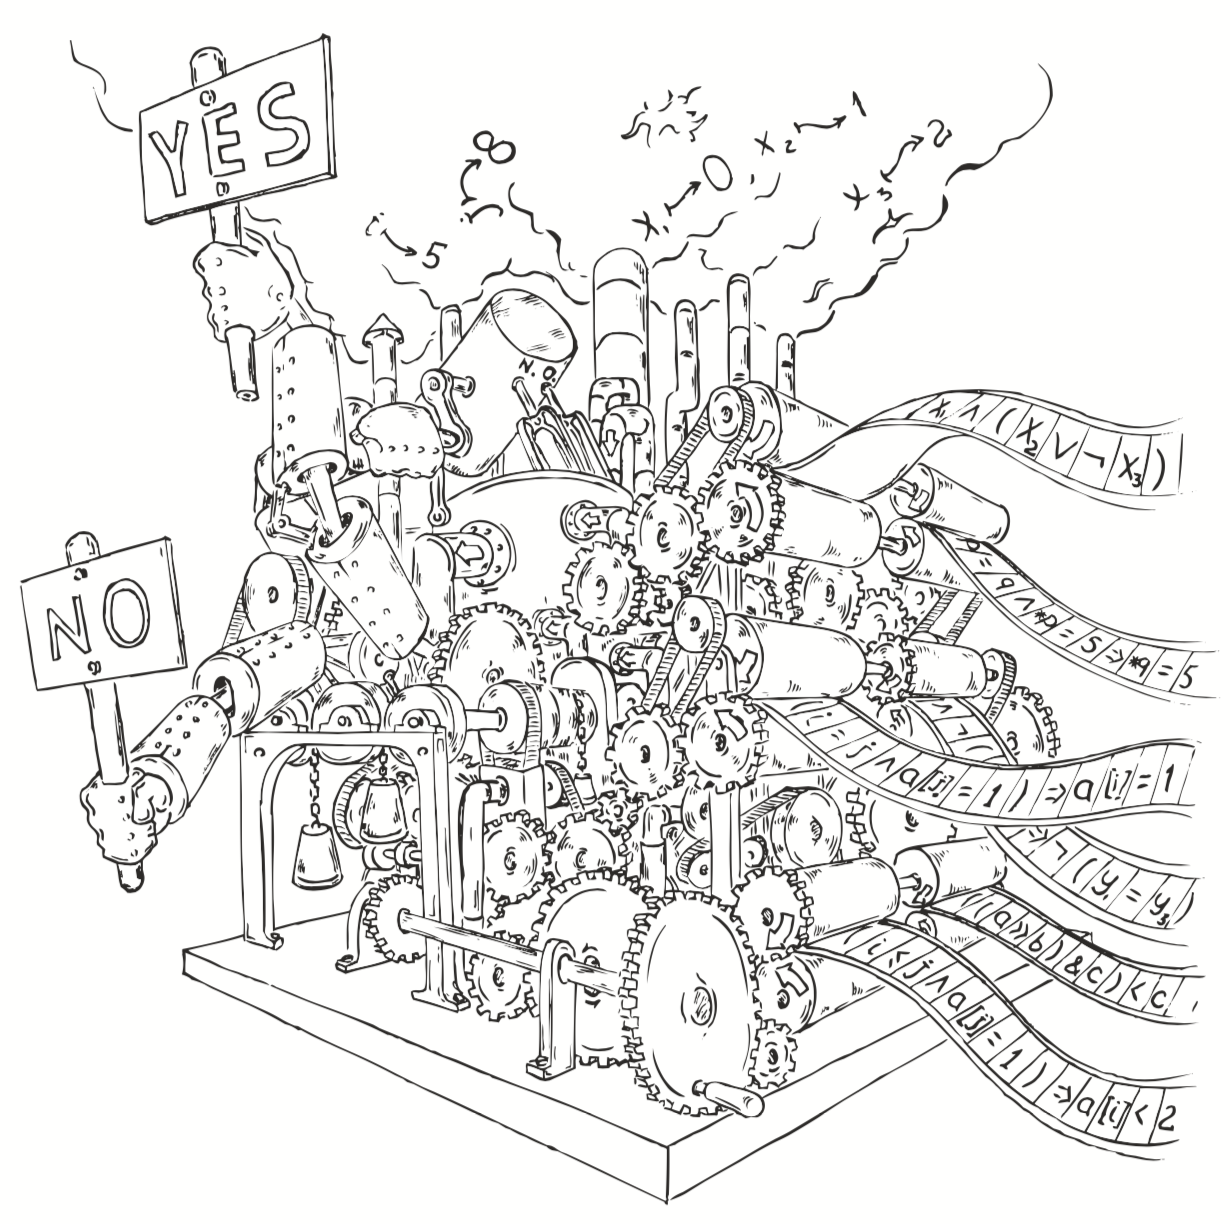
\includegraphics[scale=0.5]{../decision-procedure.png}
\end{frame}

\frame{\titlepage}

\begin{frame}{Логика равенства (EQ)}
$formula: formula \vee formula | \lnot formula | (formula) | atom$\newline
$atom: term = term$\newline
$term: identifier | constant$\newline
\end{frame}

\begin{frame}{Логика равенства (EQ)}
$formula: formula \vee formula | \lnot formula | (formula) | atom$\newline
$atom: term = term$\newline
$term: identifier | constant$\newline
Какова сложность задачи разрешимости формулы логики равенства?\newline
\end{frame}

\begin{frame}{Логика равенства (EQ)}
$formula: formula \vee formula | \lnot formula | (formula) | atom$\newline
$atom: term = term$\newline
$term: identifier | constant$\newline
Какова сложность задачи разрешимости формулы логики равенства?\newline
Зачем изучать и пропозиционную логику и логику равенства?\newline
\end{frame}

\begin{frame}{Удаление констант}
$\phi = \phi'$\newline
В $\phi'$ заменить все $c_i$ на $C_{c_i}$\newline
Для всех $i \neq j$ добавить в $\phi'$ формулы $C_{c_i} \neq C_{c_j}$
\end{frame}

\begin{frame}{Удаление констант}
$\phi' = \phi$\newline
В $\phi'$ заменить все $c_i$ на $C_{c_i}$\newline
Для всех $i \neq j$ добавить в $\phi'$ формулы $C_{c_i} \neq C_{c_j}$\newline
Далее будем считать, что в логике нет констант
\end{frame}

\begin{frame}{Логика неинтерпретируемых функций (UF)}
$F(x) = F (G(y)) \vee x + 1 = y$\newline
\end{frame}

\begin{frame}{Логика неинтерпретируемых функций (UF)}
$F(x) = F (G(y)) \vee x + 1 = y$\newline
$formula: formula \vee formula | \lnot formula | (formula) | atom$\newline
$atom: term = term| predicate\_symbol(list\_of\_terms)$\newline
$term: identifier | function\_symbol(list\_of\_terms)$\newline
\end{frame}

\begin{frame}{Логика неинтерпретируемых функций (UF)}
$F(x) = F (G(y)) \vee x + 1 = y$\newline
$formula: formula \vee formula | \lnot formula | (formula) | atom$\newline
$atom: term = term| predicate\_symbol(list\_of\_terms)$\newline
$term: identifier | function\_symbol(list\_of\_terms)$\newline
Если predicate\_symbol состоит только из \{=\}, то логику называют EUF
\end{frame}

\begin{frame}{Логика неинтерпретируемых функций(UF)}
Как используется?\newline
\end{frame}

\begin{frame}{Логика неинтерпретируемых функций(UF)}
Как используется?\newline
Если можем доказать в этой логике, то можем доказать и в общей фомруле
\end{frame}

\begin{frame}{Логика неинтерпретируемых функций(UF)}
Как используется?\newline
Если можем доказать в этой логике, то можем доказать и в общей фомруле\newline
Главное, чтобы выполнялось условие функциональной совместимости: значение функции на одних и тех же аргументах одинаково
\end{frame}

\begin{frame}{Логика неинтерпретируемых функций(UF)}
Как используется?\newline
Если можем доказать в этой логике, то можем доказать и в общей фомруле\newline
Главное, чтобы выполнялось условие функциональной совместимости: значение функции на одних и тех же аргументах одинаково\newline
Обратное не верно: если формула не тавтология в EUF, то не факт, что это не тавтология в EUF
\end{frame}

\begin{frame}{Эквивалентность программ}
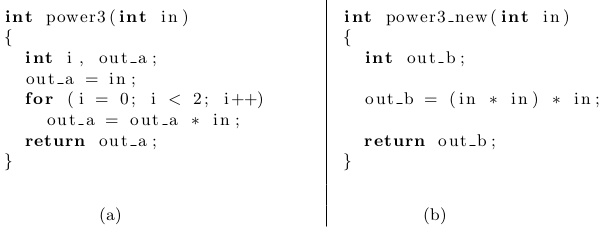
\includegraphics[scale=0.5]{power3.png}
\end{frame}

\begin{frame}{Эквивалентность программ}
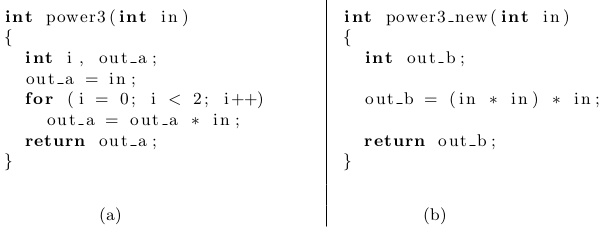
\includegraphics[scale=0.5]{power3.png}
$\phi_a := (out\_a_0 = in\_a_0) \wedge (out\_a_1 = out\_a_0 * in\_a_0) \wedge (out\_a_2 = out\_a_1 * in\_a_0)$\newline
$\phi_b := out\_b_0 = (in\_b_0 * in\_b_0) * in\_b_0$\newline
Чтобы программы были эквивалентны, должно выполняться:\newline
$(in\_a_0 = in\_b_0) \wedge \phi_a \wedge \phi_b \rightarrow out\_a_2 = out\_b_0$
\end{frame}

\begin{frame}{Эквивалентность программ}
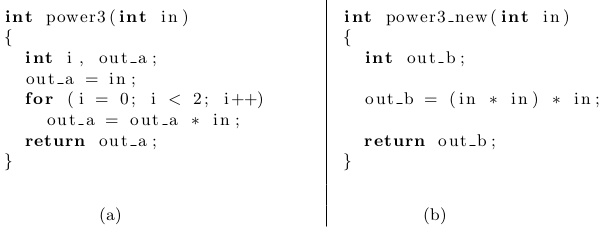
\includegraphics[scale=0.5]{power3.png}
Перепишем формулу в EUF. Будем считать, что * - это некоторый двуместный функциональный символ G(,)
\end{frame}

\begin{frame}{Эквивалентность программ}
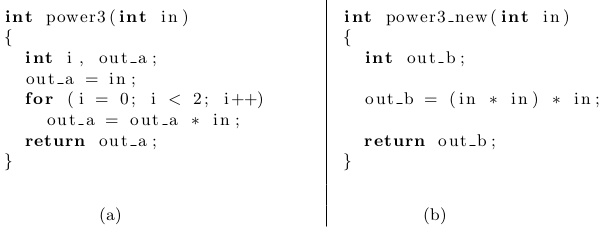
\includegraphics[scale=0.5]{power3.png}
Перепишем формулу в EUF. Будем считать, что * - это некоторый двуместный функциональный символ G(,)
$\phi_a := (out\_a_0 = in\_a_0) \wedge (out\_a_1 = G(out\_a_0, in\_a_0)) \wedge (out\_a_2 = G(out\_a_1, in\_a_0)$\newline
$\phi_b := out\_b_0 = G(G(in\_b_0, in\_b_0), in\_b_0)$\newline
Чтобы программы были эквивалентны, должно выполняться:\newline
$(in\_a_0 = in\_b_0) \wedge \phi_a \wedge \phi_b \rightarrow out\_a_2 = out\_b_0$, но теперь нам не нужно знать природу G
\end{frame}

\begin{frame}{Эквивалентность программ}
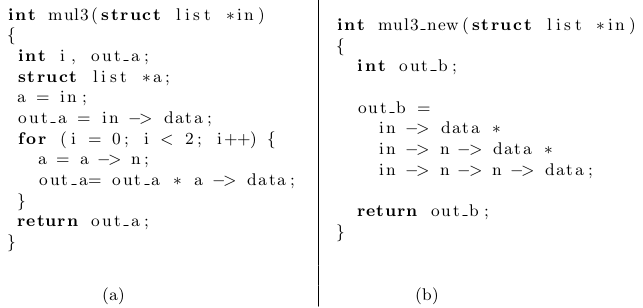
\includegraphics[scale=0.5]{mul3.png}
\end{frame}

\begin{frame}{Эквивалентность программ}
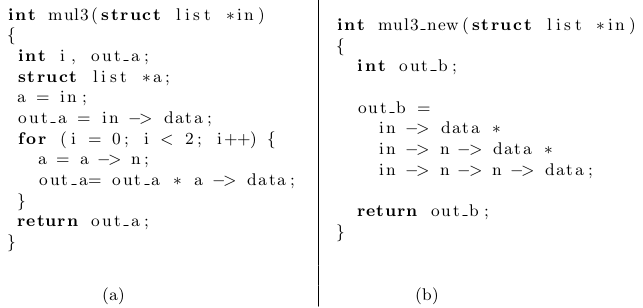
\includegraphics[scale=0.5]{mul3.png}
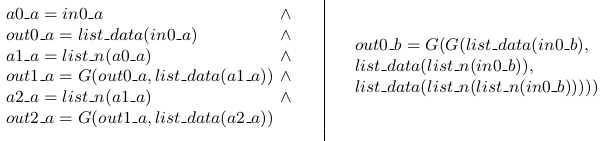
\includegraphics[scale=0.5]{mul3_ans.png}
\end{frame}

\begin{frame}{Замыкание классов эквивалентности}
\begin{itemize}
\item Построить замыкание классов эквивалентности:\newline
Поместить в один класс эквивалентности термы, если $t_1 = t_2$\newline
Слить все в один класс эквивалентности формулы $F(t_i)$, такие что $F(t_i) = F(t_j)$ и $t_i$ и $t_j$ в одном классе
эквивалентности\newline
Повторять, пока есть что сливать
\item Если какие-то $\phi_i$ и $\phi_j$ в одном классе эквивалентности и есть неравенство $\phi_i \neq \phi_j$, то вернуть результат
<<Unsatisfiable>>. Иначе вернуть <<Satisfiable>>
\end{itemize}
\end{frame}

\begin{frame}{Пример}
$(x_1 = x_2) \wedge (x_2 = x_3) \wedge (x_4 = x_5) \wedge (x_5 \neq x_1) \wedge (F(x_1) \neq F(x_3))$
\end{frame}

\begin{frame}{Недостаточность функциональной совместимости}
$(x_1 = y_2) \wedge (x_2 = y_1) \rightarrow (x_1 + y_1) = (x_2 + y_2)$
\end{frame}

\begin{frame}{Алгоритм уточнения}
\begin{enumerate}
\item $\phi' = t(\phi)$ (t - абстрагирование исходной формулы)
\item если $\phi'$ - тавтология, то исходная так же тавология
\item если $\phi' = \phi$, то не тавтология
\item добавить "уточнение" и вернуться на шаг 2
\end{enumerate}
\end{frame}

\begin{frame}{Пример}
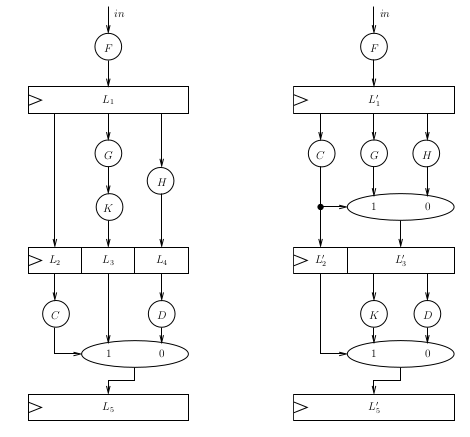
\includegraphics[scale=0.5]{circuit.png}
\end{frame}

\begin{frame}{Пример}
$z = (x_1 + y_1) * (x_2 + y_2)$\newline
$u_1 = x_1 + y_1; u_2 = x_2 + y_2; z = u_1 * u_2$
\end{frame}

\begin{frame}
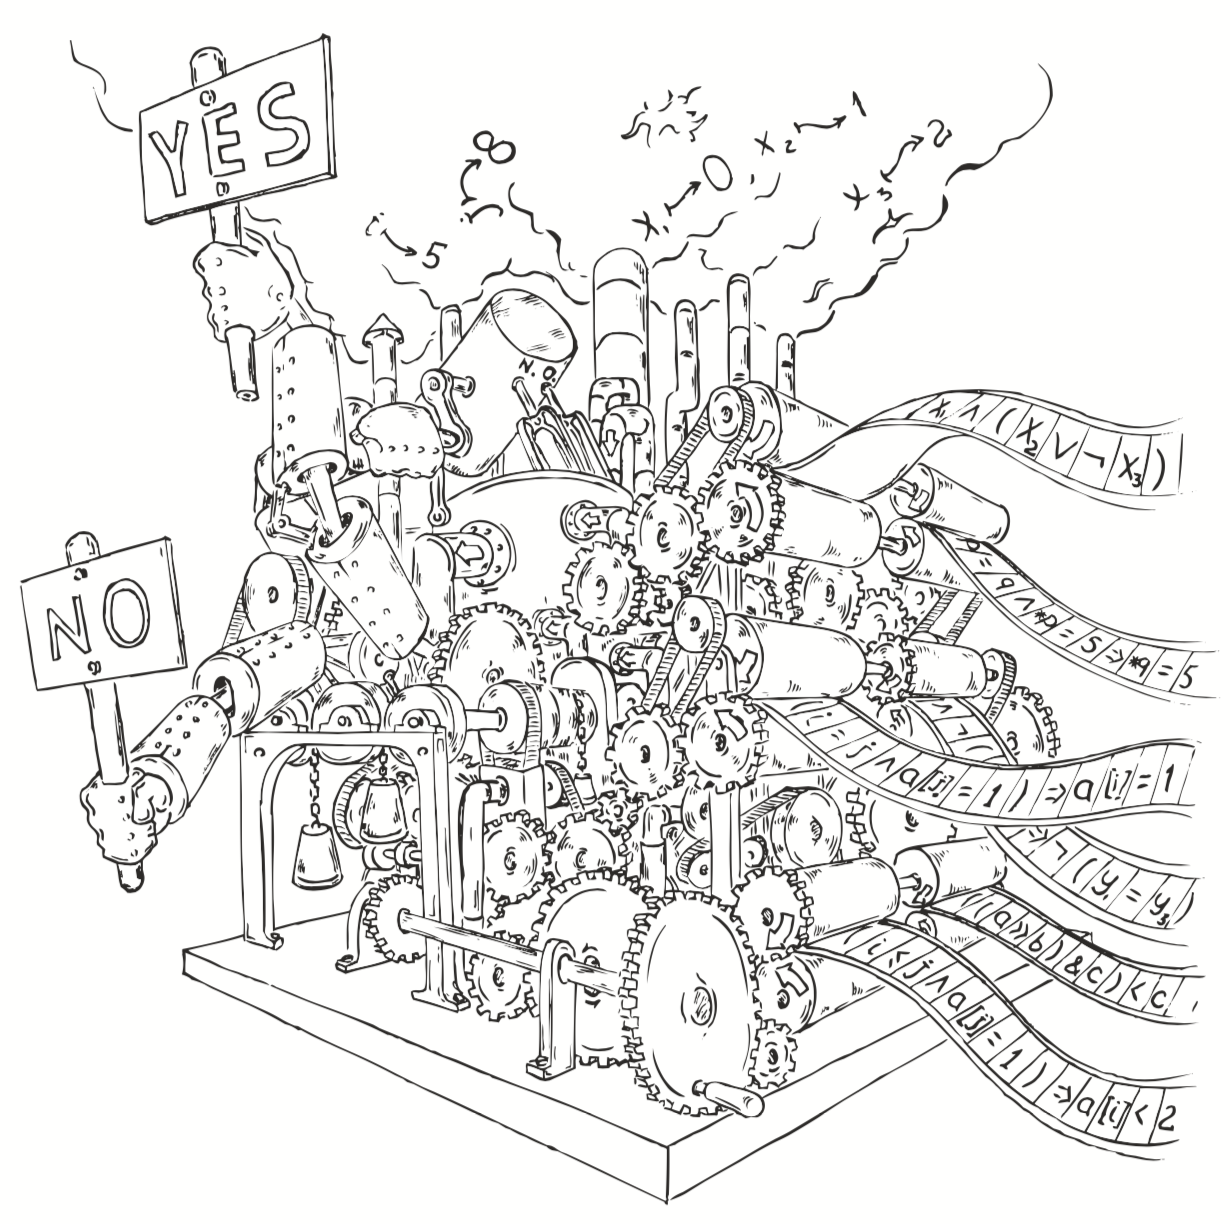
\includegraphics[scale=0.5]{../decision-procedure.png}
\end{frame}

\end{document}
